\message{ !name(lecture2.Rnw)}%%% Title:    DSBG Stats & Methods: Lecture 2
%%% Author:   Kyle M. Lang
%%% Created:  2017-MAY-19
%%% Modified: 2017-SEP-06

\documentclass{beamer}
\usetheme[%
  pageofpages          = of,
  bullet               = circle,
  titleline            = true,
  alternativetitlepage = true,
  titlepagelogo        = Logo3,
  watermark            = watermarkTiU,
  watermarkheight      = 100px,
  watermarkheightmult  = 4%
]{UVT}

\usepackage{graphicx}
\usepackage[natbibapa]{apacite}
\usepackage[libertine]{newtxmath}

%% Ensure styles of `blocks' (used in Definitions, Theorems etc.) follows the
%% UVT-style theme:
\setbeamercolor{block title}{fg = darkblue, bg = white}
\setbeamercolor{block body}{use = block title, bg = block title.bg}

%% Ensure TableOfContents is in UVT-style theme:
\setbeamercolor{section in toc}{fg = darkblue}

\title{Simple Linear Regression}
\subtitle{Statistics \& Methodology Lecture 2}
\author{Kyle M. Lang}
\institute{Department of Methodology \& Statistics\\Tilburg University}
\date{September 7, 2017}

\newcommand{\R}{\textsf{R}}

\begin{document}

\message{ !name(lecture2.Rnw) !offset(-3) }


<<setup, include=FALSE>>=
set.seed(235711)
library(knitr)
library(ggplot2)
library(plyr)
opts_chunk$set(size = 'footnotesize', fig.align = 'center')
knit_theme$set('edit-kwrite')

lightBlue <- rgb(0, 137, 191, max = 255)
midBlue   <- rgb(0, 131, 183, max = 255)
darkBlue  <- rgb(0, 128, 179, max = 255)
deepGold  <- rgb(184, 138, 45, max = 255)
lightGold <- rgb(195, 146, 48, max = 255)
@


\begin{frame}[t,plain]
\titlepage
\end{frame}


\begin{frame}{Outline}

  \begin{enumerate}
  \item Introduction to the ``regression'' problem
    \va
  \item Simple linear regression
    \va
  \item Model evaluation, hypothesis testing
  \end{enumerate}

\end{frame}


\begin{frame}{Regression Problem}

  \emph{Regression} problems (as opposed to \emph{classification} problems)
  involve modeling a quantitative response.
  \va
  \begin{itemize}
  \item The simple mean comparison we've been considering is a type of
    regression problem.
    \vb
    \begin{itemize}
    \item Although the independent variable (IV; phone type) is qualitative, the
      dependent variable (DV; rating) is quantitative.
    \end{itemize}
    \va
  \item The regression problem begins with a random outcome variable, $y$.
    \va
  \item We hypothesize that the mean of $Y$ is dependent on some set of
    covariates, $\mathbf{X}$.
  \end{itemize}

\end{frame}

\watermarkoff

\begin{frame}{Regression Models}

  \begin{columns}
    \begin{column}{0.5\textwidth}
      The distributions we've considered thus far imply a constant mean.
      \va
      \begin{itemize}
      \item Each observation is expected to have the same value of $Y$,
        regardless of their individual characteristics.
        \va
      \item This type of distribution is called ``marginal'' or ``unconditional.''
      \end{itemize}
    \end{column}
    
    \begin{column}{0.5\textwidth}
      
<<echo = FALSE, cache = TRUE>>=
x <- seq(-4.0, 4.0, 0.001)

dat2 <- data.frame(X = x, density = dnorm(x))

p1 <- ggplot(dat2, aes(x = X, y = density)) + theme_classic() +
    coord_cartesian(xlim = c(-4, 4)) +
    theme(text = element_text(size = 16, family = "Courier"))

p1 + geom_line() +
    geom_vline(xintercept = 0, linetype = "dotted", size = 2)
@

\end{column}
\end{columns}

\end{frame}


\begin{frame}{Regression Models}
  
  \begin{columns}
    \begin{column}{0.5\textwidth}
      The distributions we consider in regresssion problems have
      \emph{conditional means}.
      \va
      \begin{itemize}
      \item The value of $Y$ that we expect for each observation is defined by
        the observations' individual characteristics.
        \va
      \item This type of distribution is called a ``conditional.''
      \end{itemize}
    \end{column}
    
    \begin{column}{0.5\textwidth}
      
      \begin{figure}
        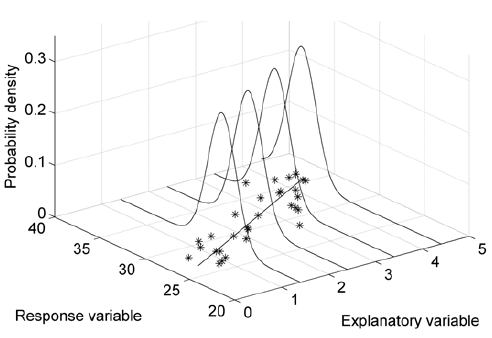
\includegraphics[width = \textwidth]{%          
          figures/conditional_density_figure.png%
        }
        \caption{\tiny{Image retreived from:
            \url{http://www.seaturtle.org/mtn/archives/mtn122/mtn122p1.shtml}}}
      \end{figure}
      
    \end{column}
  \end{columns}
  
\end{frame}


\begin{frame}{Regression Models}
  
  \begin{columns}
    \begin{column}{0.5\textwidth}
      We've already seen one conditional distribution visualized.
      \va
      \begin{itemize}
      \item One curve corresponds to ratings from observations of Phone A while
        the other comes from observations of Phone B.
        \va
      \item With a qualitative explanatory variable, it doesn't make sense to
        use a 3D plot.
      \end{itemize}
    \end{column}
    
    \begin{column}{0.5\textwidth}
            
    \end{column}
  \end{columns}
  
\end{frame}

\watermarkon

\begin{frame}{Simple Linear Regression}
\end{frame}


\begin{frame}{Differences from Correlation}
\end{frame}


\begin{frame}{Evaluating Regression Models}
\end{frame}


\begin{frame}{Testing Hypotheses}
\end{frame}


\begin{frame}{Effect Size}
\end{frame}


\begin{frame}{Assumptions}
\end{frame}



%\begin{frame}[allowframebreaks]{References}
%
%  \bibliographystyle{apacite}
%  \bibliography{../../bibtexStuff/statMethRefs.bib}
%
%\end{frame}


\end{document}


\message{ !name(lecture2.Rnw) !offset(-227) }
